The exact `quasi-optimal' scheme for building a tensor train is TT-SVD~\cite{tensortrain}, where the first two steps for a 4-way tensor are illustrated in~\cref{fig:ttsequence}. As shown, This simply involves a series of reshape operations (permutations) followed by skinny SVDs. Provided that reshape operations can be efficiently performed in distributed memory (or avoided altogether), we can implement this method efficiently in distributed memory (using a `Gram' style SVD approach, as in~\cref{alg:sthosvd}). This would be the first know distribute implementation of a tensor train decomposition.

Furthermore, both common solution methods for computing a tensor train decomposition (SVD or optimization) may be able to efficiently leverage the previously discussed ideas from randomized SVD and randomized least squares, respectively. Thus we propose to explore the following questions:

\begin{itemize}
\item Can `sweeping' optimization algorithms for the tensor train be written in a way that can leverage randomized least squares, e.g., as described in~\cref{sec:sketching}?
\item Can the SVD method for forming the tensor train decomposition be expressed in a way that can be efficiently performed in distributed memory? E.g., starting from the distributed tensor representation outlined in~\cref{sec:tucker}.
\item Can ideas from randomized low-rank decompositions be applied efficiently to this formulation in distributed memory? E.g., using methods from~\cite{tropp2}. 
\end{itemize}

\begin{figure}
  \centering 
  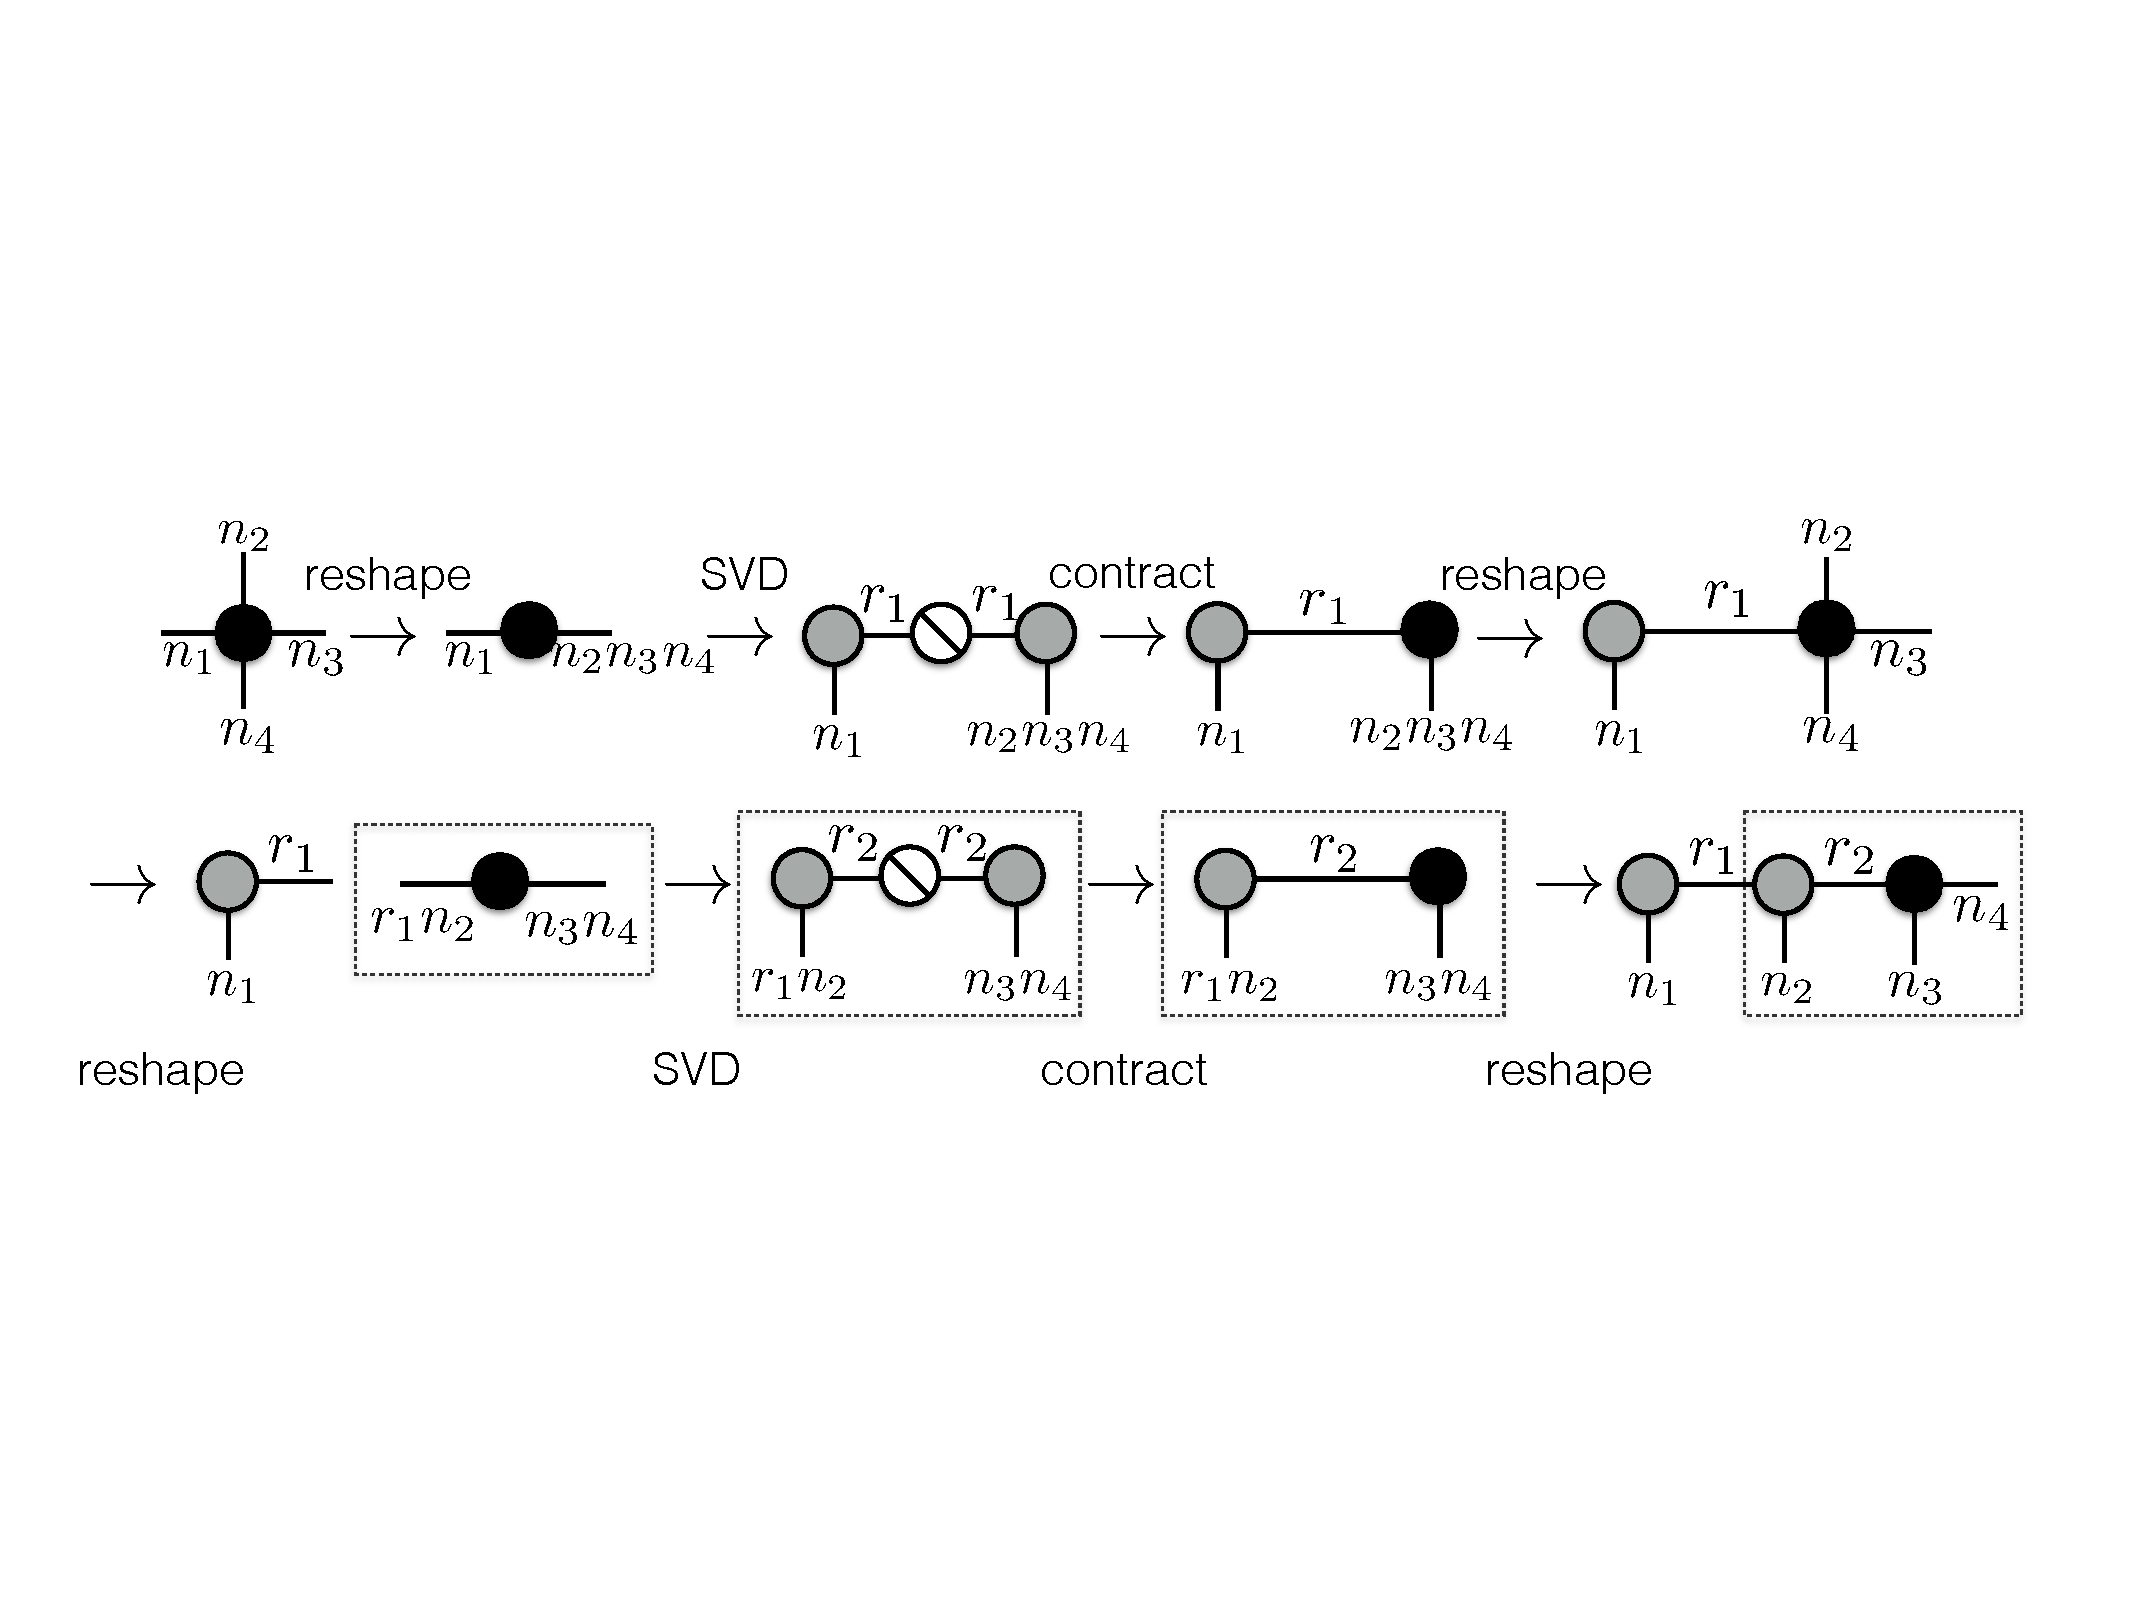
\includegraphics[width=\linewidth]{thpropfigs/ttsequence}
  \caption{The creation of the first two `carriages' of a tensor train decomposition for a 4-way tensor.}
  \label{fig:ttsequence}
\end{figure}

\paragraph{Proposal}
We summarize our proposed contributions as follows:
\begin{itemize}
  \item Implement the first distributed-memory implementation of the tensor train decomposition.
  \item Analyze the communication and computation behavior of the `reshape-SVD' method in distributed memory.
  \item Apply methods from our randomized Tucker decomposition to the tensor train in distributed memory.
  \item Benchmark both methods on a supercomputer and analyze/establish tradeoffs.
\end{itemize}